%All of this chapter should be removed eventually
\section{How to get the most out of this template} \label{cha:how-to-template}
This section is aimed to help you using this template. It does not aim to teach you how to use \LaTeX as there are plenty of resources that would do a far more effective job. Some places to start are included in section \ref{sec:latex_resources}.

Instead the aim here is is to help a relatively inexperienced \LaTeX user navigate the template, point them to places they can learn more, give some helpful hints and examples of cool stuff you can do.

\subsection{Setting up this template}

\subsubsection{Template}
You can use the code behind this project as your starting point, however, you will have to go through the process of removing all the guidance text. It may therefore be more advisable to use the blank template to start and then use this as your reference.

If you do choose to use this document as your starting point you can remove this chapter (no. \ref{cha:how-to-template}) by taking out the input command in \verb|main.tex| that refers to this file and the \verb|guidance-example-section| folder.

\subsubsection{Metadata}
Your first steps upon starting working with this template should be to edit lines \numrange{6}{11} in \verb|main.tex|. They should currently read as:

\begin{minted}[]{latex}
% Document metadata
% fill these in to update header, footer and titlepage
\def\modulename{Module Name}
\def\assignmenttitle{Assignment Title}
\def\studentidnumber{Student ID Number}
\def\datesubmitted{Date Submitted}
\end{minted}

Replace the text in black in the squigly brackets \{\} with your details and the details of your assignment and they will be updated on the title page, header and footer through the document.

\subsubsection{Style}
This template has been set up to best match the university style and uses appropriate fonts, logos, etc.

The University also has a published house style guide \parencite{uniofbirmingham2024housestyleguide} that may prove useful. For example the following guidance is given for headings:

\begin{quote}
    Headings should always be in sentence case and without a full stop. This is an initial capital followed by all lower case (unless a proper noun appears in the heading). This includes left-hand navigation bars on the web. Use sentence case for events. Do not use initial capitals for emphasis anywhere.
\end{quote}

\subsection{\LaTeX resources} \label{sec:latex_resources}
You are obviously free to use any service or setup to edit and compile your \LaTeX documents but we would recommend Overleaf (as of Nov. 2024). It is web based so you don't need to install software and you should be able to access it from any computer. There is also a professional license for all students and staff in EPS (College of Engineering and Physical Sciences) accessed through UoB single sign-on.

Here are some handy starting points for getting started with \LaTeX for you to explore.

\begin{itemize}
    \item Overleaf Documentation \parencite{overleaf-documentation}
        \begin{itemize}
            \item As well as being a good option for managing your \LaTeX projects, the documentation and guidance provided by Overleaf is rather good.
            \item A good starting point may be the learn \LaTeX in 30 minutes guide \url{www.overleaf.com/learn/latex/Learn_LaTeX_in_30_minutes}
        \end{itemize}
    \item ShareLaTeX YouTube Guides \parencite{youtube-sharelatex-channel}
        \begin{itemize}
            \item A youtube channel recommended by the University library service that provides a number of guides.
            \item \url{https://www.youtube.com/@ShareLaTeX/videos}
        \end{itemize}
    \item University resources
        \begin{itemize}
            \item There are often events through the year that are useful for getting started with LaTeX. There is a planned lecture as an introduction in the Engineering Department.
            \item The University Computer Science Society (CSS) and Hacking Society (AFNOM)  run a series of lunchtime lectures through the year called the missing semester \parencite{missing-semester}, this included a session on \LaTeX  the notes for which can be found at:  \url{https://missingsemester.afnom.net/2024/latex/}
        \end{itemize}
\end{itemize}

\subsection{Some interesting examples of things \LaTeX can do}

\subsubsection{Referencing}
For documents produced for the MSc it is a requirement to use Harvard style referencing (Author-Date), luckily \LaTeX can handle remove most of the headache normally associated with managing references. This document template is setup to cite and produce a bibliography inline with these requirements.

It may be a good idea to manage your references with a reference manager, some examples of these are Zotero, EndNote or Mendeley. All will export your references in a \verb|.bib| file which \LaTeX can read. If you are using Overleaf then at the time of writing there are integrations for both Zotero and Mendeley which enable library syncing which may be a nice feature for you.

Once you have a bib file it is very simple to create a citation, for Harvard style \verb|\parencite| cites in brackets, \verb|\textcite| is inline text, \verb|\autocite| tries to make the choice based on context. 

The references section at the end of the document is created through the \verb|\printbibliography| command at the end of the document and will include only the citations made in the document.

\subsubsection{Numbers and units}
\verb|siunitx| is a package that allows for better number and unit typesetting. The full documentation gives an excellent guide \parencite{wright2024siunitx} but here are a few examples as a starting point.

Here are some examples of typesetting numbers:
\begin{itemize}
    \item \num{125}
    \item \num{12345}
    \item \num{1.2e34}
    \item \num{1.2e-3}
    \item \ang{12.34}
    \item \numlist{1;23;4567}
    \item \numrange{90}{125}
\end{itemize}

Here are some examples of typesetting units, they can either be input in math style or interpreted:
\begin{itemize}
    \item \unit{km/hr}
    \item \unit{kg.m/s^2}
    \item \unit{m/s}
    \item \unit{\metre \per \second}
    \item \unit{\square\volt\cubic\lumen\per\farad}
\end{itemize}

Units and numbers can then be combined together in qty:
\begin{itemize}
    \item Speed of light ($c$): 
        \begin{itemize}
            \item \qty{299792458}{m.s^{-1}}
            \item \qty{3.0e8}{\metre\per\second}
        \end{itemize}
    \item Planck constant ($h$): 
        \begin{itemize}
            \item \qty{6.63e-34}{J.Hz^{-1}}
        \end{itemize}
    \item Newtonian constant of gravitation ($G$): 
        \begin{itemize}
            \item \qty{6.67e-11}{m^3.kg^{-1}.s^{-2}}
        \end{itemize}
    \item \qtyrange{90}{125}{mph}
    \item \qtylist{30;45;70;90;150}{\km \per \hour}
\end{itemize}

\subsubsection{Figures}

\begin{figure}[H]
    \centering
    
\includegraphics[width=0.3\linewidth]{images/uob_logo.pdf}
    \caption{University of Birmingham Logo}
    \label{fig:uob_logo}
\end{figure}

This template uses the \verb|graphicx| package for figures. Figure \ref{fig:uob_logo} is a example of a  basic image as a figure.

\begin{figure}[H]
    \centering
    \begin{subfigure}[b]{0.22\textwidth}
        \centering
        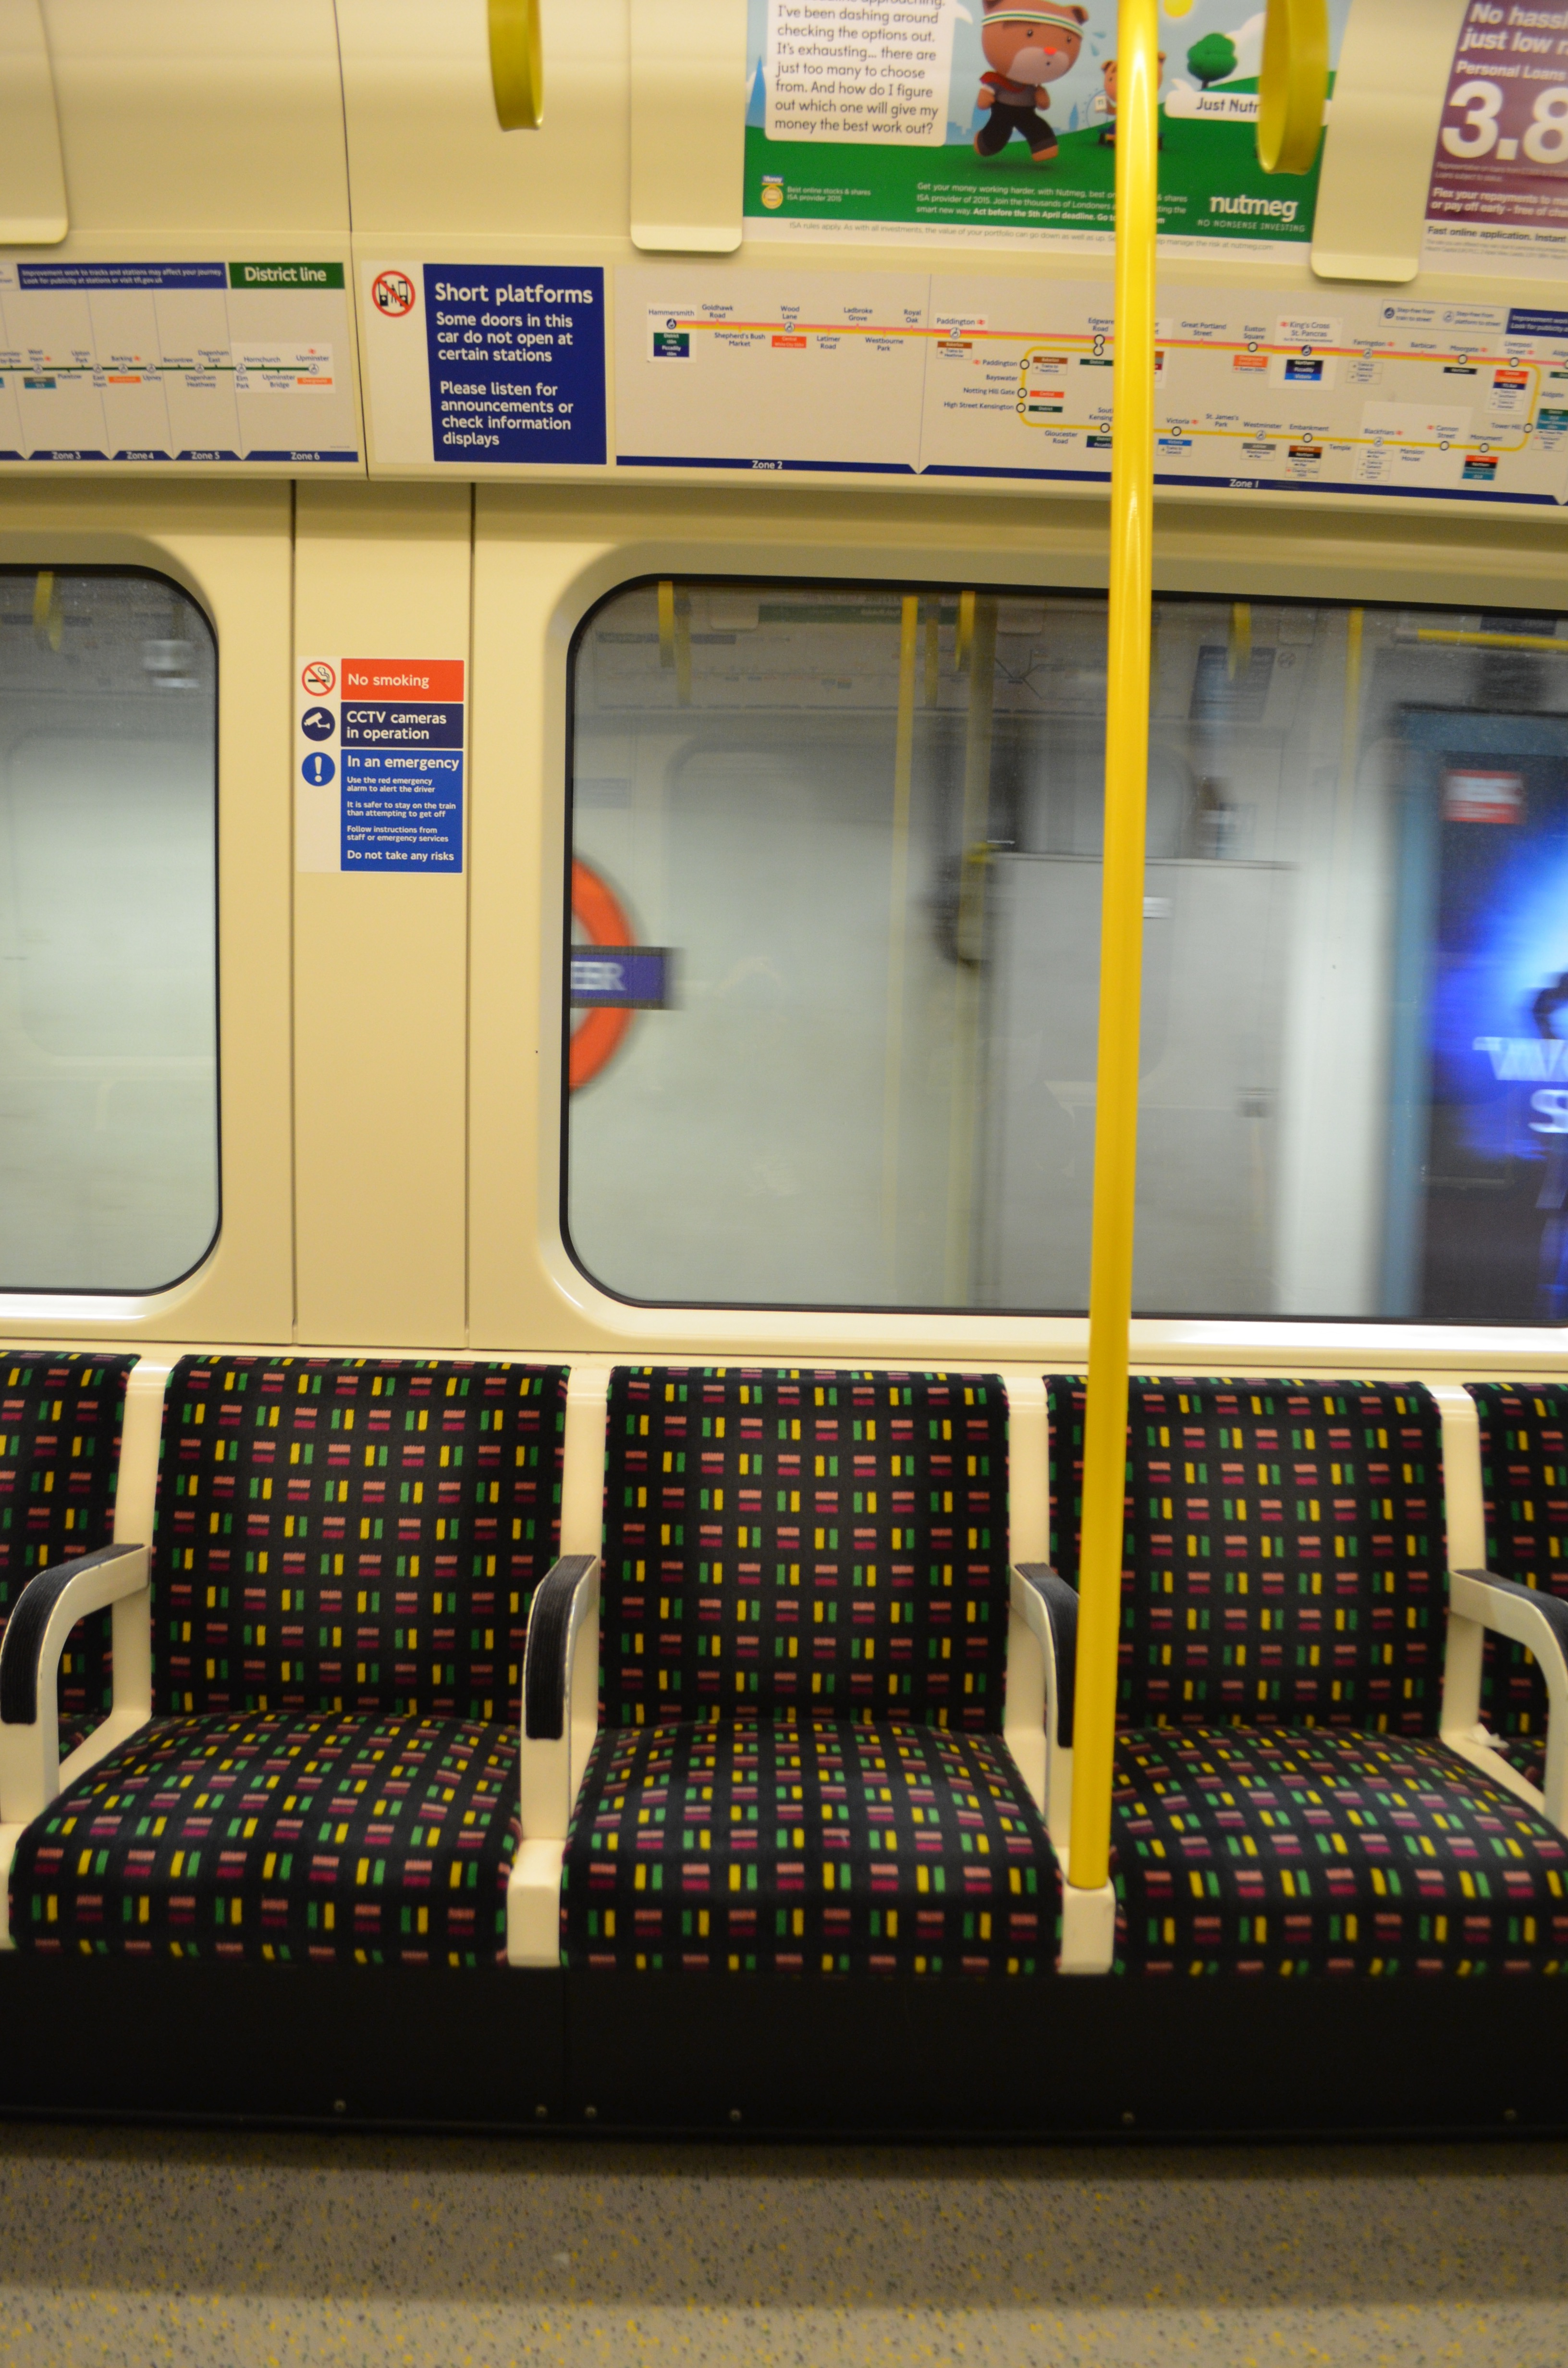
\includegraphics[width=\textwidth]{guidance/images/rathbone2017circle.jpg}
        \caption{Circle line \parencite{rathbone2017circle}}
        \label{fig:rathbone2017circle}
    \end{subfigure}
    \hfill
    \begin{subfigure}[b]{0.22\textwidth}
        \centering
        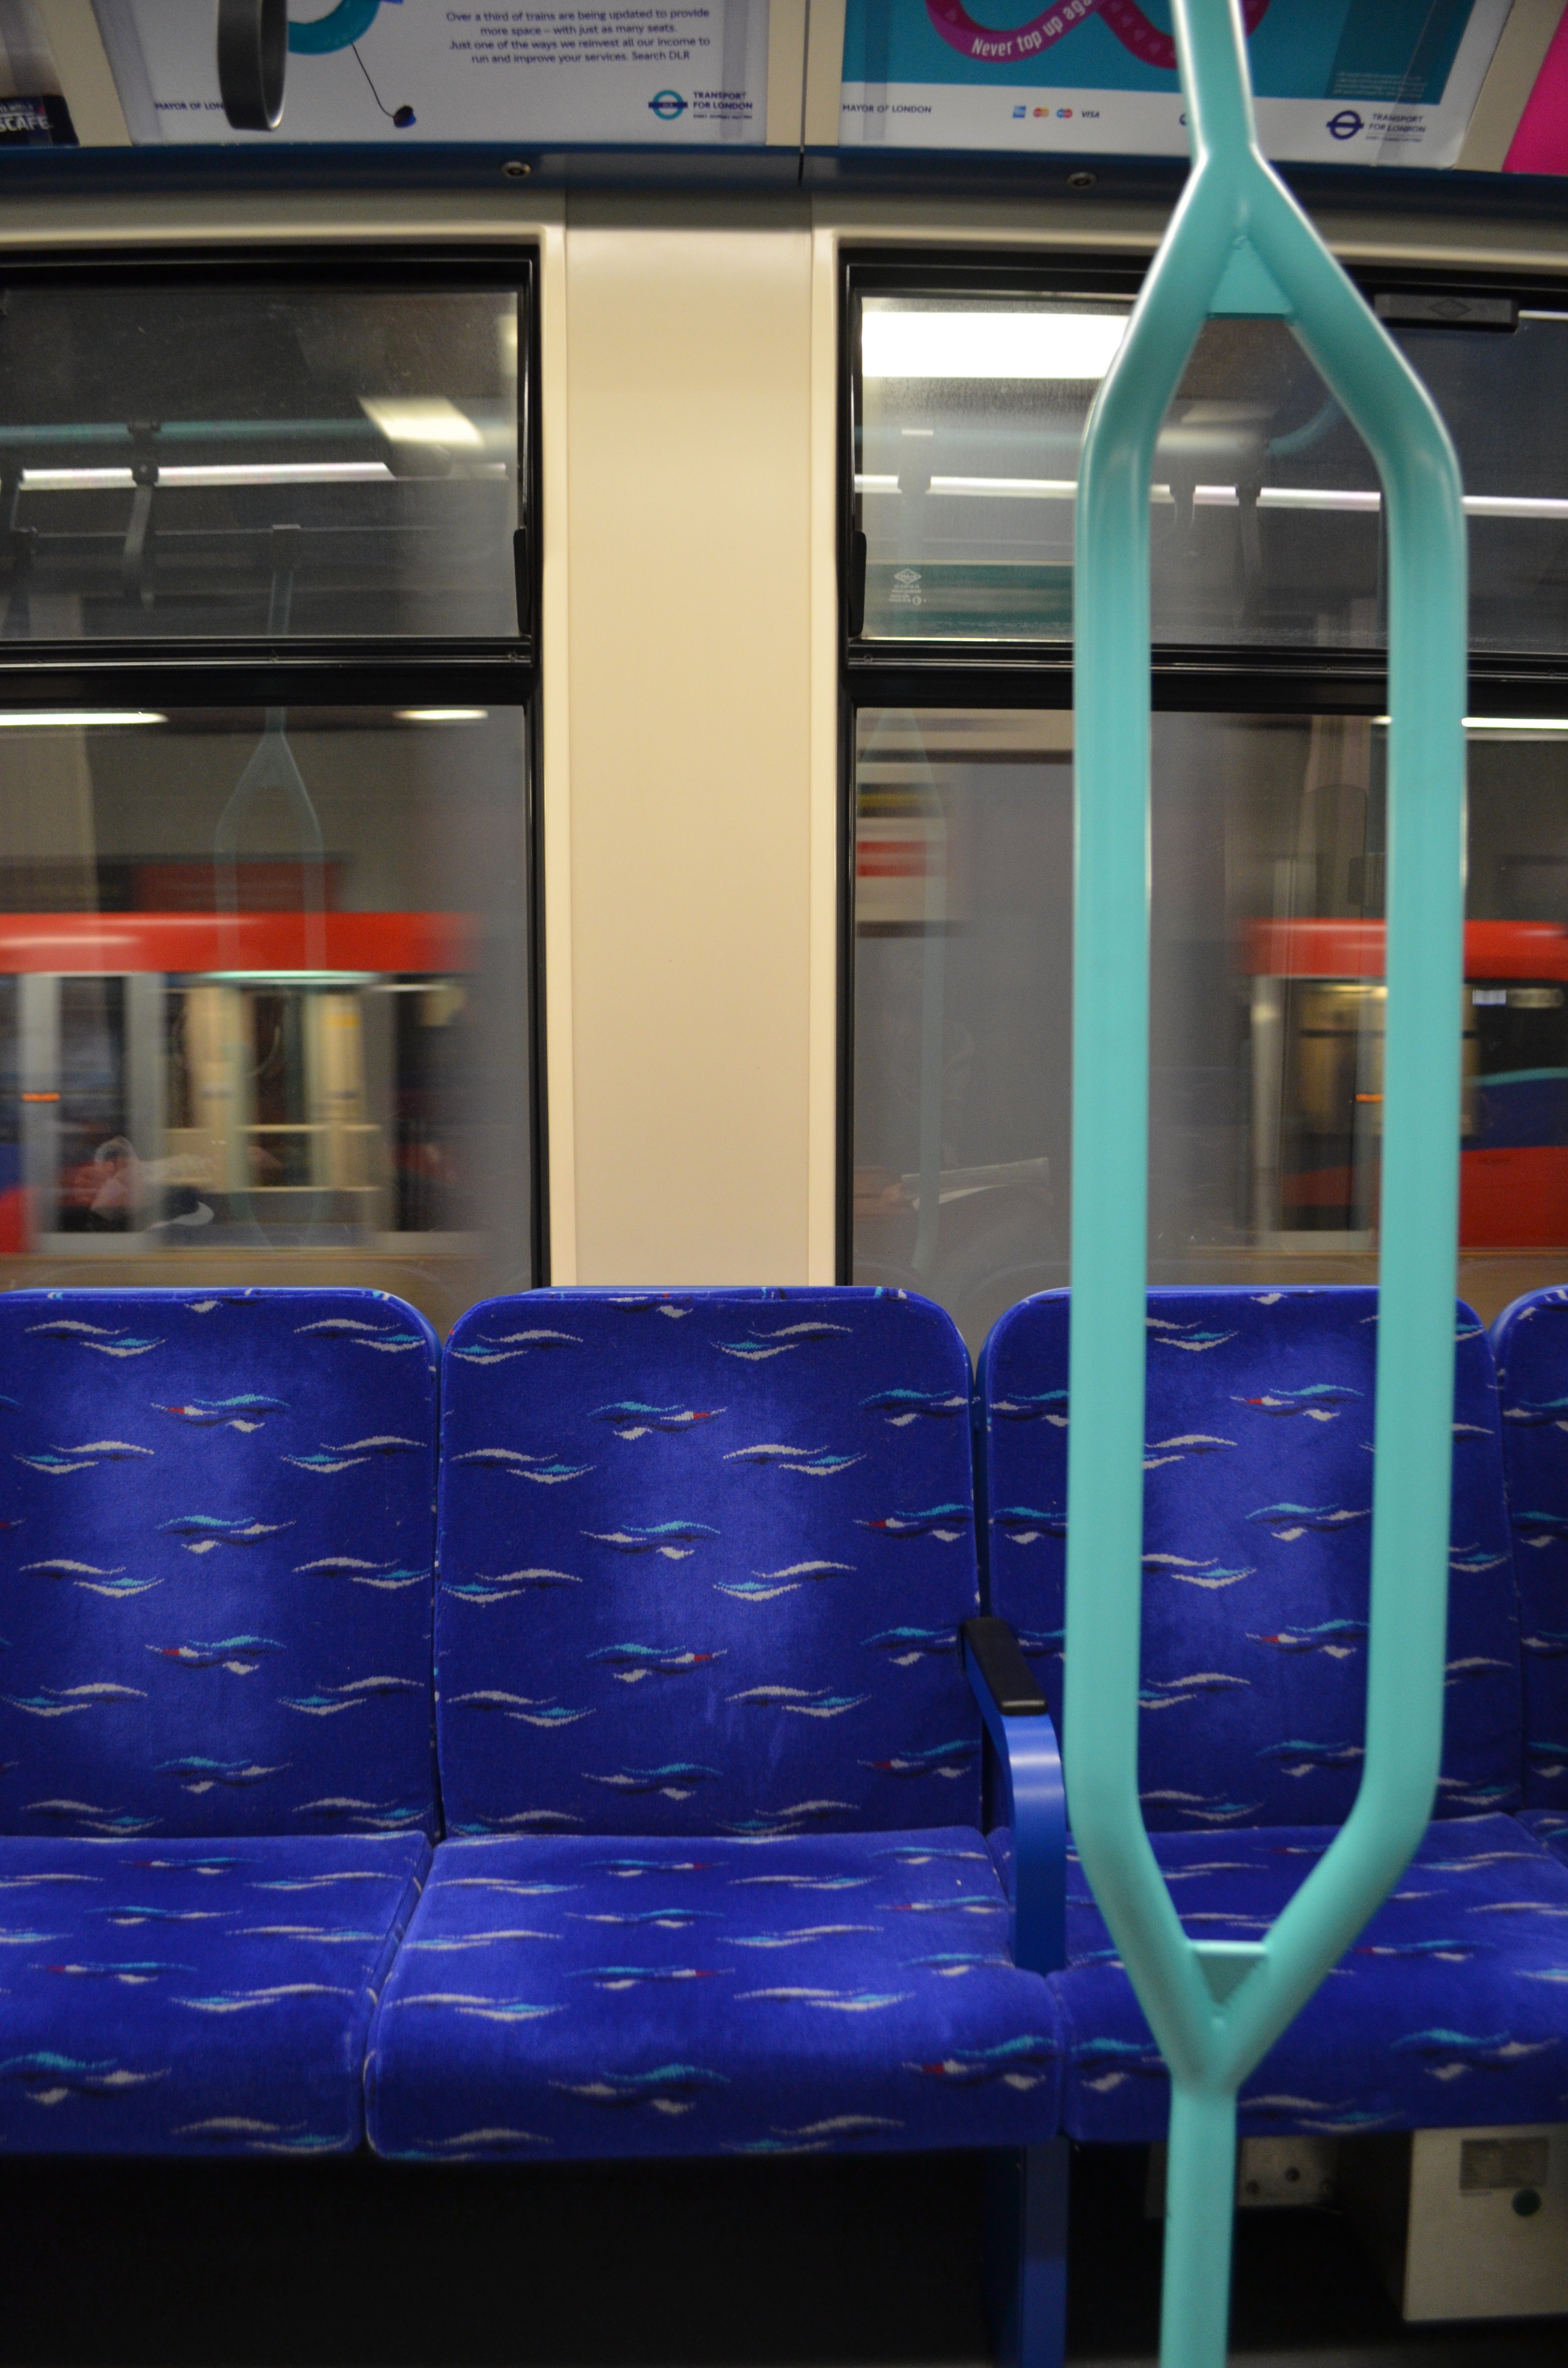
\includegraphics[width=\textwidth]{guidance/images/rathbone2017dlr.jpg}
        \caption{DLR \parencite{rathbone2017dlr}}
        \label{fig:rathbone2017dlr}
    \end{subfigure}
    \hfill
    \begin{subfigure}[b]{0.22\textwidth}
        \centering
        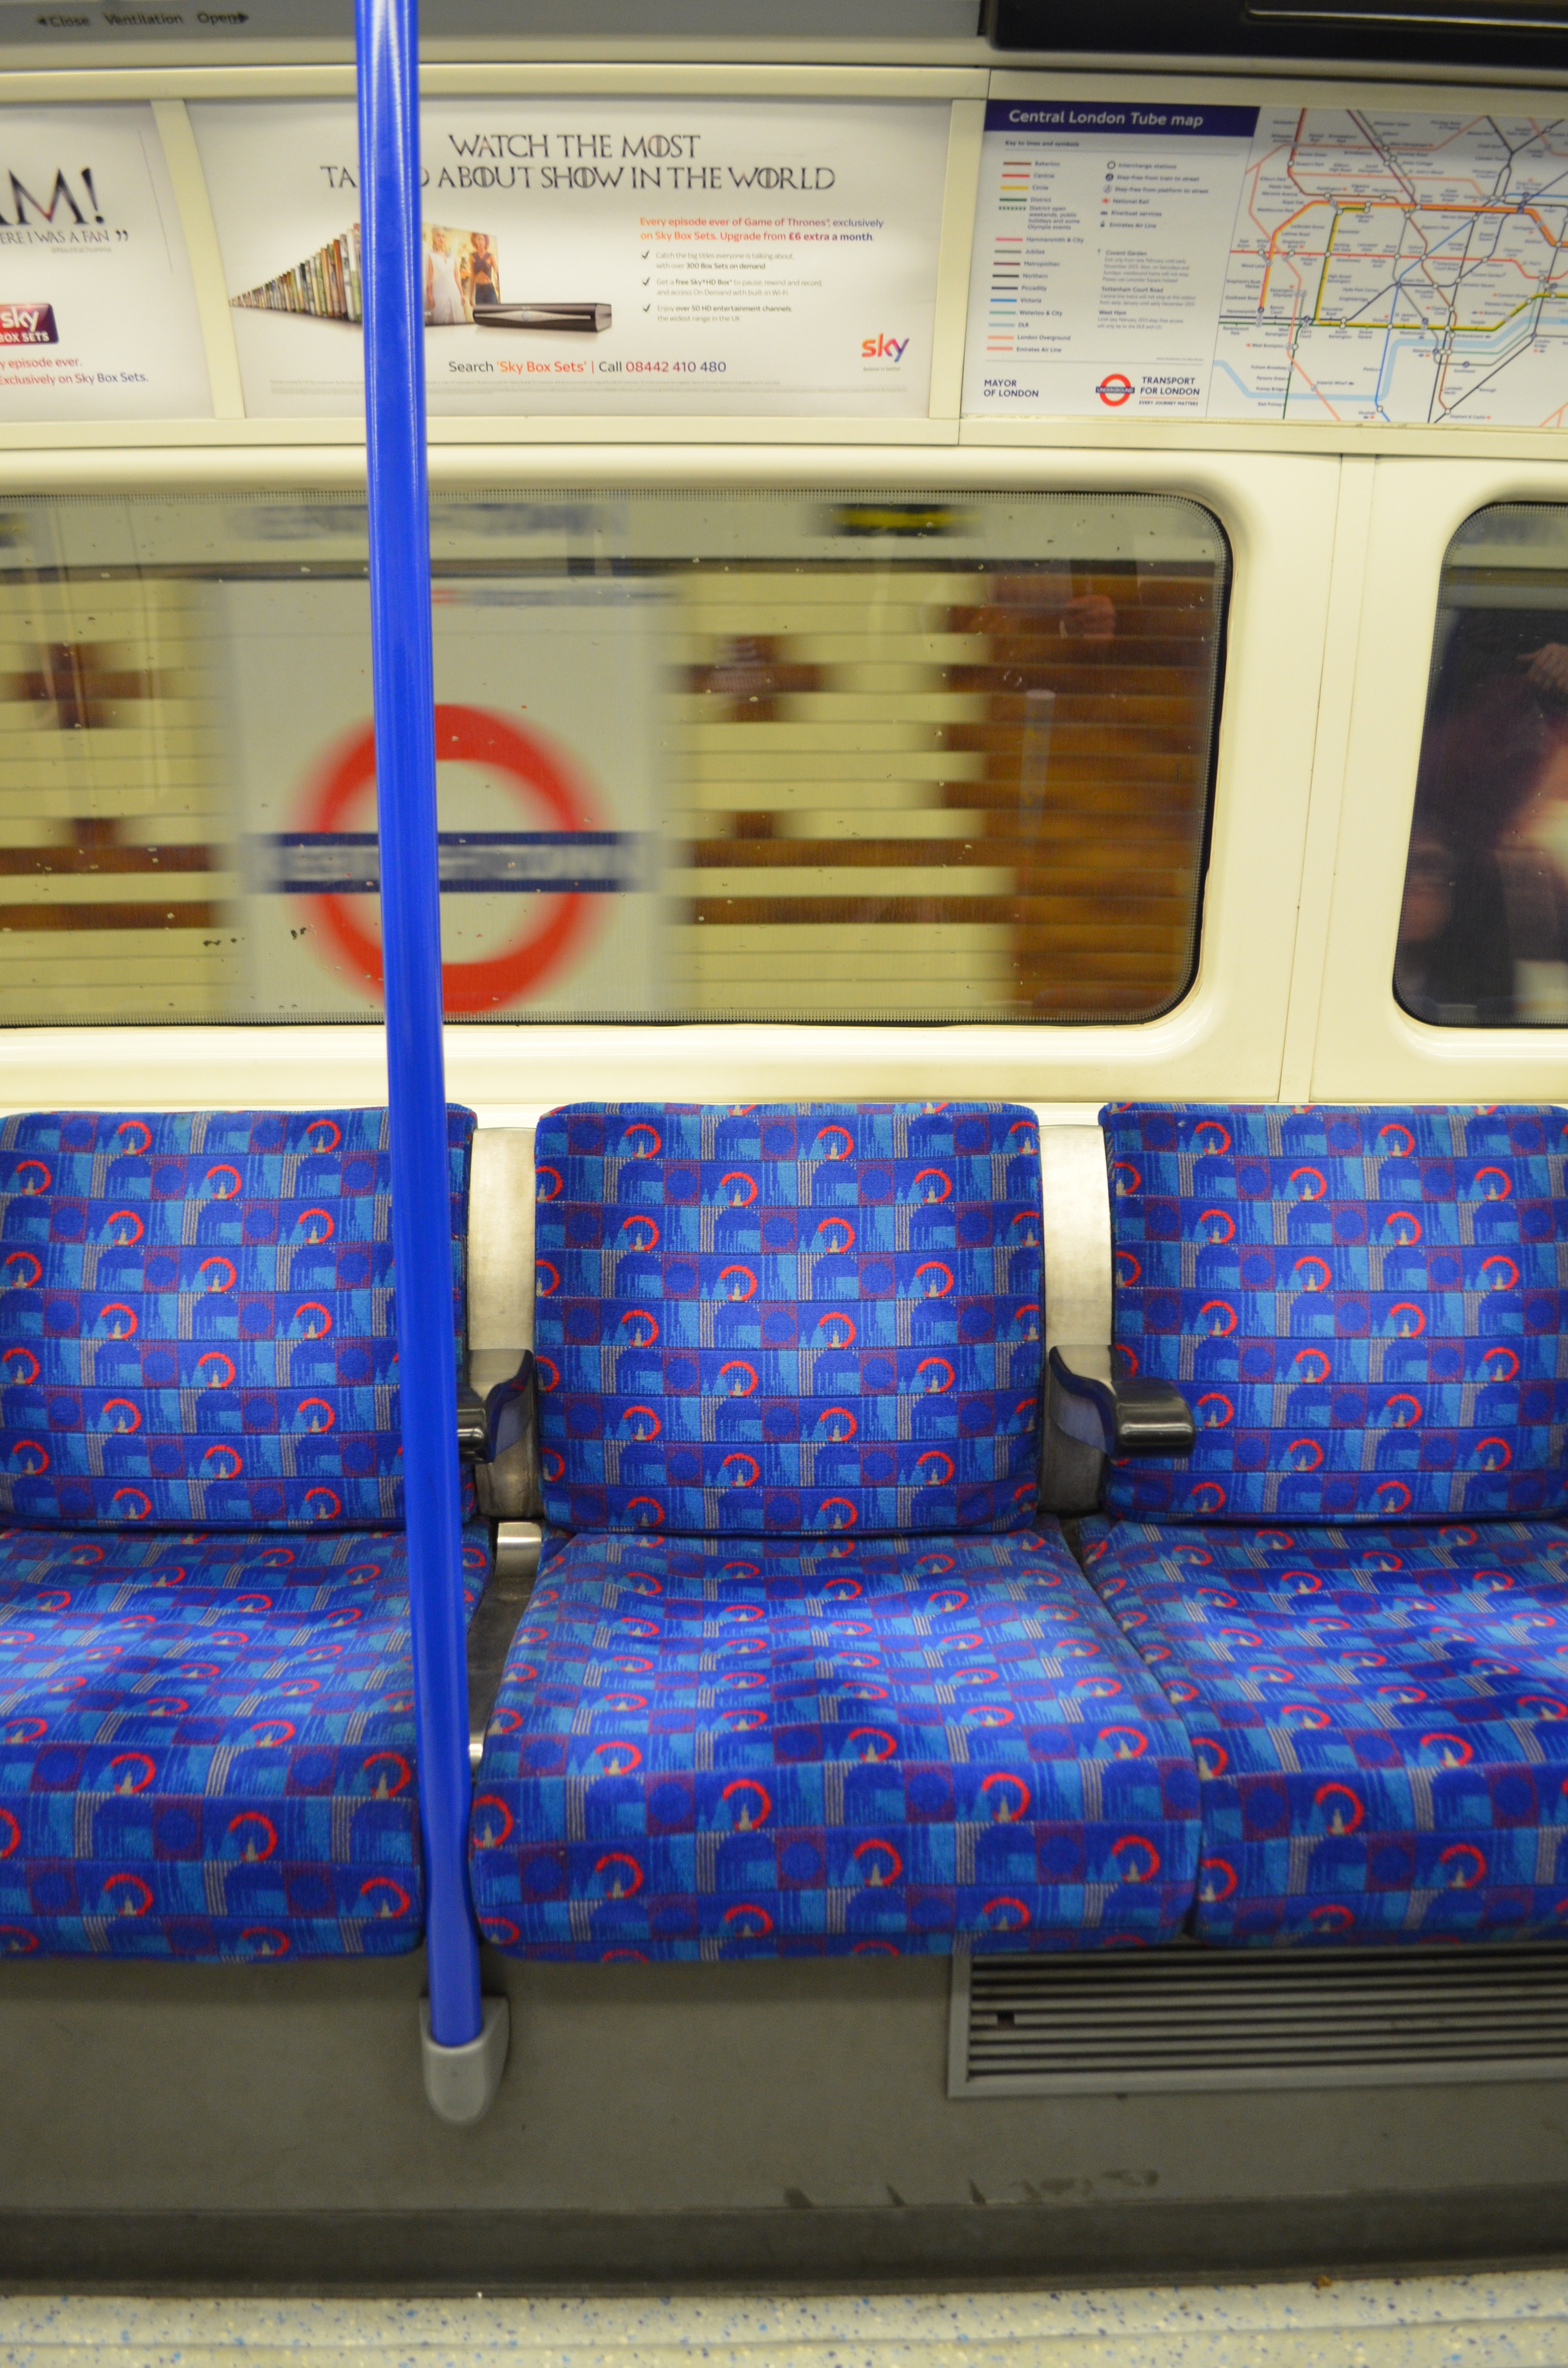
\includegraphics[width=\textwidth]{guidance/images/rathbone2017northern.jpg}
        \caption{Northern line \parencite{rathbone2017northern}}
        \label{fig:rathbone2017northern}
    \end{subfigure}
    \hfill
    \begin{subfigure}[b]{0.22\textwidth}
        \centering
        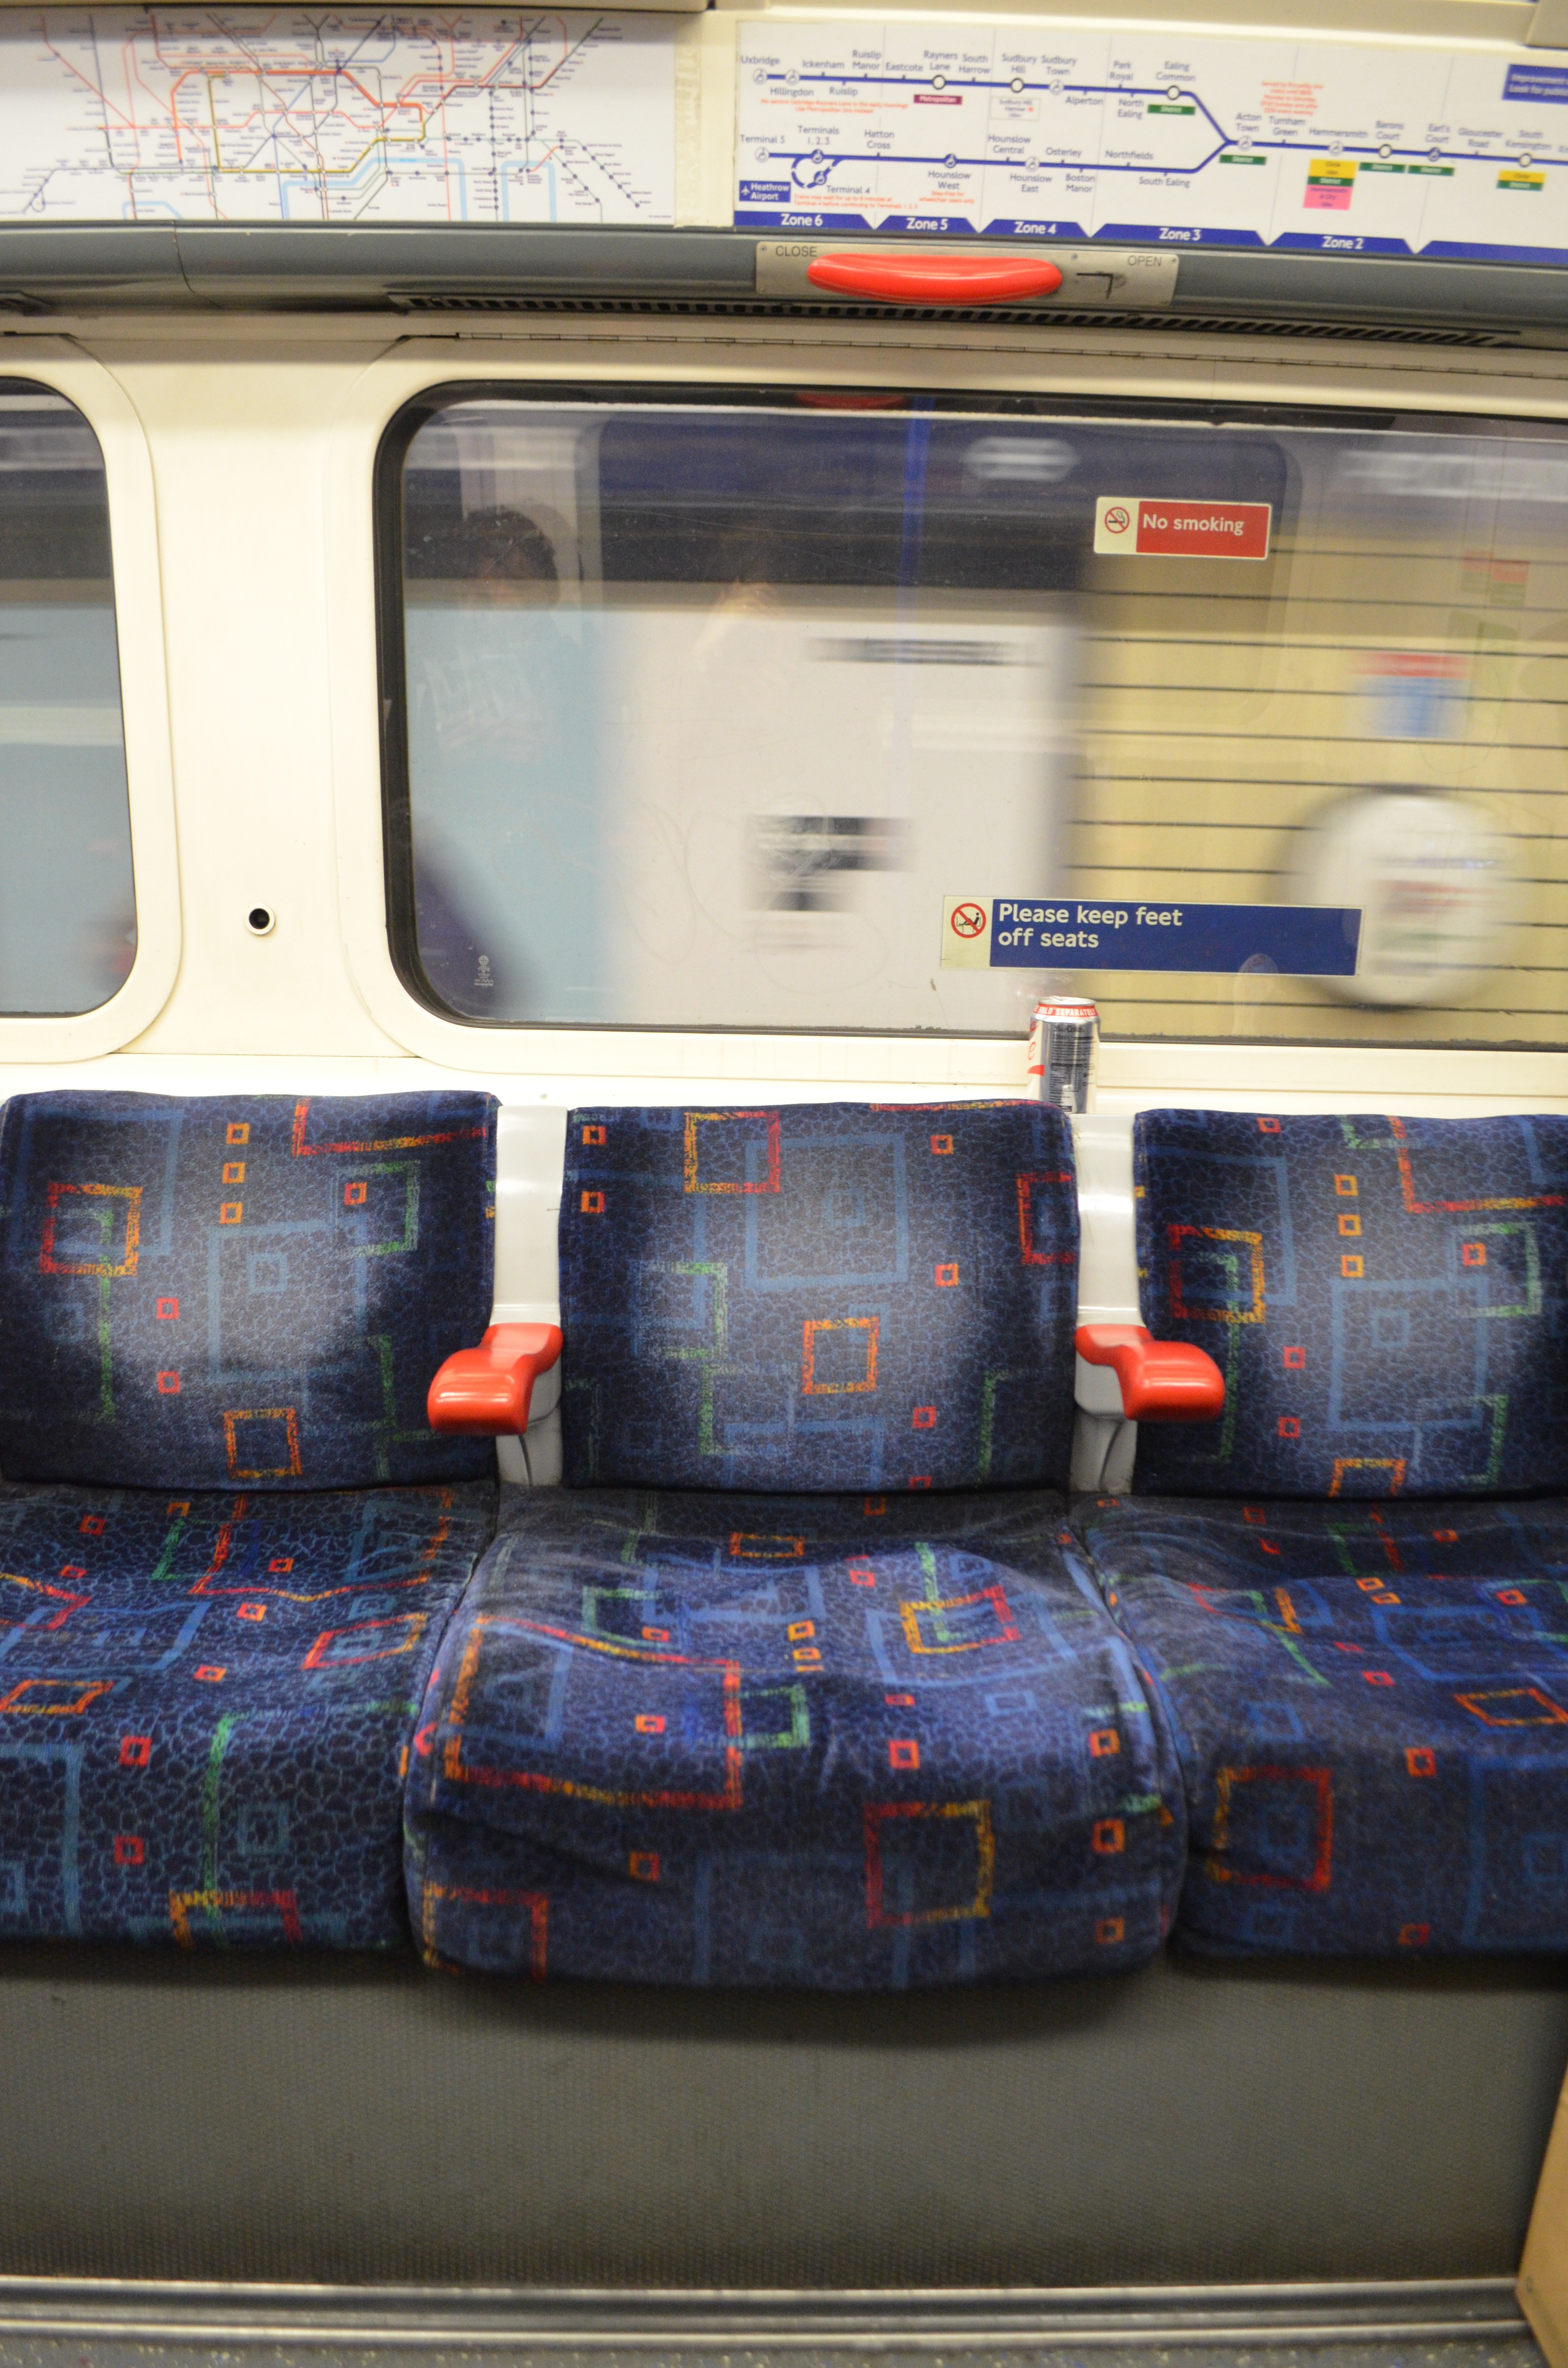
\includegraphics[width=\textwidth]{guidance/images/rathbone2017piccadilly.jpg}
        \caption{Piccadilly line \parencite{rathbone2017piccadilly}}
        \label{fig:rathbone2017piccadilly}
    \end{subfigure}
    \caption{4 examples of Transport for London seat cover patterns or "Moquettes". Courtesy of Loughborough University, accessed 10 October, 2024, \url{https://repository.lboro.ac.uk/projects/Transport_for_London_seat_cover_patterns/24400}}
    \label{fig:rathbone2017}
\end{figure}

Figure \ref{fig:rathbone2017} is a slightly more complicated figure. It is a single figure that contains the sub figures \ref{fig:rathbone2017circle}, \ref{fig:rathbone2017dlr}, \ref{fig:rathbone2017northern} and \ref{fig:rathbone2017piccadilly}. For more complex sections of code for large figures like this is can be useful to store that section in a seperate \verb|.tex| file as has been done here and in subsequent plots.

\begin{figure}[H]
    \centering
    \begin{tikzpicture}
        \begin{axis}[
            width=0.8\textwidth,
            height=0.6\textwidth,
            axis lines = left,
            xlabel = {x},
            ylabel = {y},
            xmajorgrids=true,
            ymajorgrids=true,
            ymin=-1,
            ymax=1,
            xmin=0,
            xmax=7
        ]
            \addplot[color=blue] table [x=x, y=1_term, col sep=comma]{guidance-example-section/data/fourier_series_square_wave.csv};
            \addlegendentry{1 term}
            \addplot[color=red] table [x=x, y=2_term, col sep=comma]{guidance-example-section/data/fourier_series_square_wave.csv};
            \addlegendentry{2 terms}
            \addplot[color=brown] table [x=x, y=3_term, col sep=comma]{guidance-example-section/data/fourier_series_square_wave.csv};
            \addlegendentry{3 terms}
            \addplot[color=black] table [x=x, y=20_term, col sep=comma]{guidance-example-section/data/fourier_series_square_wave.csv};
            \addlegendentry{20 terms}
        \end{axis}
    \end{tikzpicture}
    \caption{Fourier series approximation of a square wave with varying number of cosine terms. Plotted with pgfplots from stored csv data}
    \label{fig:fourier_series_square_wave_csv}
\end{figure}

\begin{figure}[H]
    \centering
    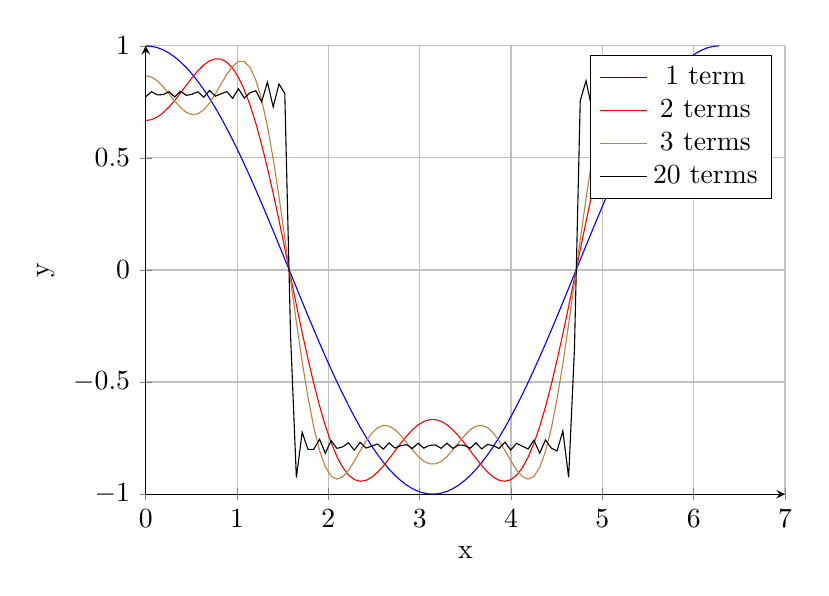
\begin{tikzpicture}
        \begin{axis}[
            width=0.8\textwidth,
            height=0.6\textwidth,
            axis lines = left,
            xlabel = {x},
            ylabel = {y},
            xmajorgrids=true,
            ymajorgrids=true,
            ymin=-1,
            ymax=1,
            xmin=0,
            xmax=7
        ]
            \addplot[
                domain=0:6.28,
                samples=100,
                color=blue
            ] {cos(x*57.2958)};
            \addlegendentry{1 term}

            \addplot[
                domain=0:6.28,
                samples=100,
                color=red
            ] {cos(x*57.2958) - (cos(3*x*57.2958)/3)};
            \addlegendentry{2 terms}

            \addplot[
                domain=0:6.28,
                samples=100,
                color=brown
            ] {cos(x*57.2958) - (cos(3*x*57.2958)/3) + (cos(5*x*57.2958)/5)};
            \addlegendentry{3 terms}

            \addplot[
                domain=0:6.28,
                samples=100,
                color=black
            ] {
                cos(x*57.2958) - 
                (cos(3*x*57.2958)/3) + 
                (cos(5*x*57.2958)/5) - 
                (cos(7*x*57.2958)/7) + 
                (cos(9*x*57.2958)/9) - 
                (cos(11*x*57.2958)/11) + 
                (cos(13*x*57.2958)/13) - 
                (cos(15*x*57.2958)/15) + 
                (cos(17*x*57.2958)/17) - 
                (cos(19*x*57.2958)/19) + 
                (cos(21*x*57.2958)/21) - 
                (cos(23*x*57.2958)/23) + 
                (cos(25*x*57.2958)/25) - 
                (cos(27*x*57.2958)/27) + 
                (cos(29*x*57.2958)/29) - 
                (cos(31*x*57.2958)/31) + 
                (cos(33*x*57.2958)/33) - 
                (cos(35*x*57.2958)/35) + 
                (cos(37*x*57.2958)/37) - 
                (cos(39*x*57.2958)/39)};
            \addlegendentry{20 terms}
        \end{axis}
    \end{tikzpicture}
    \caption{Fourier series approximation of a square wave with varying number of cosine terms. Plotted with pgfplots from functions}
    \label{fig:fourier_series_square_wave_calculated}
\end{figure}

Figures \ref{fig:fourier_series_square_wave_csv} and \ref{fig:fourier_series_square_wave_csv} both show figures plotted with the pgfplots package. Figure \ref{fig:fourier_series_square_wave_csv} is plotted from data stored in a csv file, while Figure \ref{fig:fourier_series_square_wave_calculated} is plotted directly from a set of functions. 

This can be a very useful as if you want to change the way your data is plotted (or the data that is plotted), you can change it directly in Latex without having to re-export from your tool every time.

\textbf{Image Formats}
As a rule of thumb vector images are preferable over rasterized images. \LaTeX's preferred format for vector images is \verb|.pdf| files. There are other vector formats including \verb|.svg| and \verb|.eps| which you can convert between with a bit of google assistance.

For raster images (\verb|.png|, \verb|.jpg|, etc.) the usual guidance applies, try where possible to use high quality images, especially high resolution. It is worth noting that \LaTeX allows the use of the scale command when specifying an image size which would allow the natural size or integer scaling of the natural size to maximise image quality.

If you want to learn more about image types then Adobe have produced an article that covers the difference between raster and vector images\cite{adobe-raster-vector}.


\subsubsection{Equations}
\LaTeX allows you to do inline equations, i.e. $y=mx+c$, or set on their own line, such as equations \ref{eq:1}, \ref{eq:2} and \ref{eq:3}.

\begin{equation}
    \label{eq:1}
    f(x) = 2[H \frac{x}{L} - H(\frac{x}{L} - 1)] - 1
\end{equation}

\begin{equation}
    \label{eq:2}
    \begin{split}
        b_n & = \frac{1}{L} \int_0^{2L} f(x) sin(\frac{n \pi x}{L}) dx \\
            & = \frac{4}{n \pi} 
        \begin{cases}
            0 &\text{$n$ \textit{even}} \\
            1 &\text{$n$ \textit{odd}}
        \end{cases}
    \end{split}
\end{equation}

\begin{equation}
    \label{eq:3}
    f(x) = \frac{4}{\pi} \sum_{n=1,3,5,\ldots}^\infty \frac{1}{n} sin(\frac{n \pi x}{L})
\end{equation}

\subsubsection{Tables}

\begin{table}[h]
\centering
\caption{Example simple table}
\label{tab:simple-table}
\begin{tabular}{@{}ll@{}}
\toprule
Name & Age \\ \midrule
Adam & 30 \\
Eve & 30 \\ \bottomrule
\end{tabular}
\end{table}

Table \ref{tab:simple-table} is an example of a very simple table, but there is the possibility of making them more complex, table \ref{tab:lu_line_colour_reference} has a little more data, includes some cell shading and has been placed on it's own seperate page, printed in landscape.

% table generated using https://tablesgenerator.com
\afterpage{
\clearpage
\thispagestyle{empty}
\begin{landscape}
\centering
\begin{table}
\centering
\caption{Colour Reference for London Underground lines as listed in TfL colour standard \parencite{tfl2022colourreference}}
\label{tab:lu_line_colour_reference}
\begin{tabular}{@{}lllll@{}}
\toprule
London Underground line & PMS & CMYK & RGB & Colour Sample \\ \midrule
Bakerloo line & 470 & C026 M070 Y097 K016 & R166 G090 B042 & \cellcolor[HTML]{A65A2A}{\color[HTML]{333333} } \\
Hammersmith \& City line & 197 & C003 M048 Y015 K000 & R236 G155 B173 & \cellcolor[HTML]{EC9BAD} \\
Piccadilly line & 072 & C100 M097 Y003 K003 & R000 G015 B159 & \cellcolor[HTML]{000F9F} \\
Central line & 485 & C006 M098 Y100 K001 & R225 G037 B027 & \cellcolor[HTML]{E1251B} \\
Jubilee line & 430 & C055 M041 Y038 K005 & R123 G134 B140 & \cellcolor[HTML]{7B868C} \\
Victoria line & 299 & C081 M018 Y000 K000 & R000 G160 B223 & \cellcolor[HTML]{00A0DF} \\
Circle line & 116 & C000 M018 Y100 K000 & R255 G205 B000 & \cellcolor[HTML]{FFCD00} \\
Metropolitan line & 235 & C041 M100 T041 K021 & R135 G015 B084 & \cellcolor[HTML]{870F54} \\
Waterloo \& City line & 338 & C055 M000 Y039 K000 & R107 G205 B178 & \cellcolor[HTML]{6BCDB2} \\
District line & 356 & C096 M027 Y100 K015 & R000 G121 B052 & \cellcolor[HTML]{007934} \\
Northern line & Black & C000 M000 Y000 K100 & R000 G000 B000 & \cellcolor[HTML]{000000} \\ \bottomrule
\end{tabular}
\end{table}
\end{landscape}
}




It is also possible to load data in directly from a \verb|.csv| file and then display in a table. This has been done for table \ref{tab:TSGB0101}

\begin{table}[h]
\centering
\caption{UK Passenger transport by mode, figures shown are a percentage of total passenger distance over the year \parencite{departmentoftransport2023TSGB0101}}
\label{tab:TSGB0101}
\csvautobooktabular{guidance-example-section/data/TSGB0101.csv}
\end{table}